\subsection{Βήμα 2ο - Δεδομένα από TMDb}
Στο 2ο βήμα αφού έχουμε τα δεδομένα που χρειάζονται από το πρώτο, δημιουργεί και προγραμματίζει για εκτέλεση ασύγχρονα ερωτήματα ζητώντας πλήρη δεδομένα ταινιών για κάθε αναγνωριστικό ταινίας που έχουμε στην υπηρεσία TMDb. 

Ο Στόχος δεν είναι μόνο η απόκτηση δεδομένων ταινιών αλλά και συντελεστών, εταιριών, χωρών
%χώρων?
και ειδών ταινιών, συνεπώς αφού πάρει τα δεδομένα ταινιών θα χρονοδρομολογήσει και άλλα ασύγχρονα ερωτήματα στην εν λόγω υπηρεσία για να πάρει και τα υπόλοιπα δεδομένα. 

Αφού τελειώσει αυτή η διαδικασία, συσχετίζει όλα τα δεδομένα μεταξύ τους και τα εισάγει στην βάση δεδομένων για περαιτέρω επεξεργασία από κάποιο άλλο σύστημα. 
\begin{figure}[h]
  \centering
  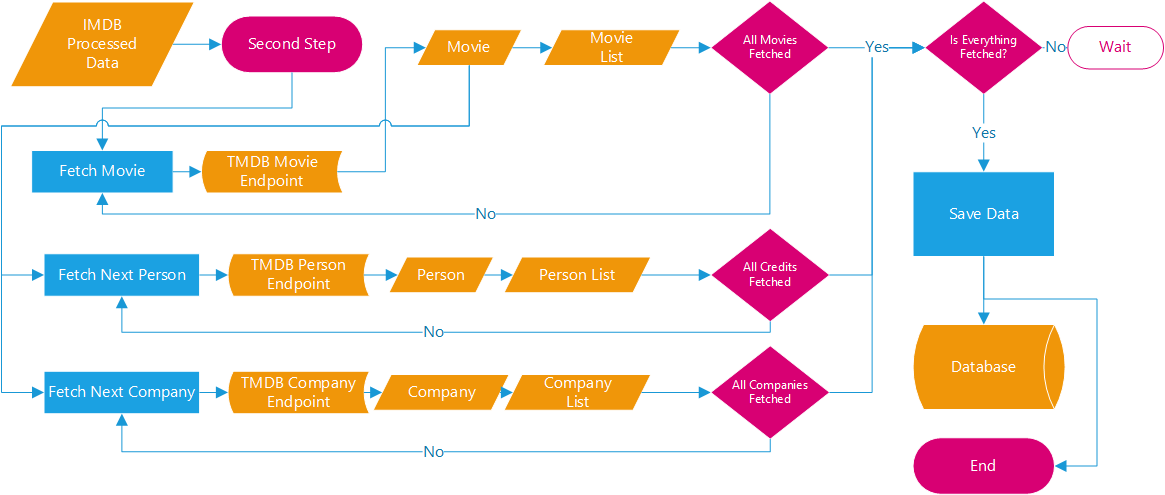
\includegraphics[width=150mm]{Chapters/5 - Architecture/Import/Images/tmdb_flowchart.png}
  \caption{Διάγραμμα ροής δεδομένων απο TMDb}
  \label{flowchart:tmdbImport}
\end{figure}